\doublespacing
\chapter{METHODOLOGY}

\section{Introduction}
\hspace{0.5in}The following sections are a detailed overview of the experiments conducted. First, training synthesis through gprMax is discussed. The topics covered are automation of training data generation and pre-processing. Then, a step by step look at the model architectures used, along with their respective loss functions, and the algorithm for training these models.

\section{Software}
\hspace{0.5in}For programming, \lstinline{python} is the only language used. All machine learning experiments were carried out with \lstinline{tf.keras} which is part of the main \lstinline{tensorflow} package \cite{tensorflow}. In addtion, for preprocessing we use \lstinline{numpy} which is part of the \lstinline{scipy} ecosystem \cite{scipy}. Finally, for visualization, we use \lstinline{matplotlib} \cite{Hunter:2007}. 

\section{Generating Training Data with GprMax}
\hspace{0.5in}To acquire training data for the GAN model, we use gprMax, an open source software to simulate electromagnetic wave propagation. It solves Maxwell’s equations in 3D using the \acrfull{fdtd} method \cite{gprMax}. We generate cylinders with diverse dielectric properties in range of substrate mixtures. For purposes of sample diversity we focus on a range of cylinder diameters in Peplinksi soil \cite{peplinski}, with a range of sand to clay ratio for each image. To provide additional randomness, we apply a seed value that is randomly selected and applied to each iteration of training data generation. Therefore, each image produced by gprMax is unique. A total of 150 A-scan traces comprise the B-scan of a single simulation as show in Figure \ref{fig:originalBscan}. 
\vspace{0.5\baselineskip}

\begin{figure}[H]
  \centering
  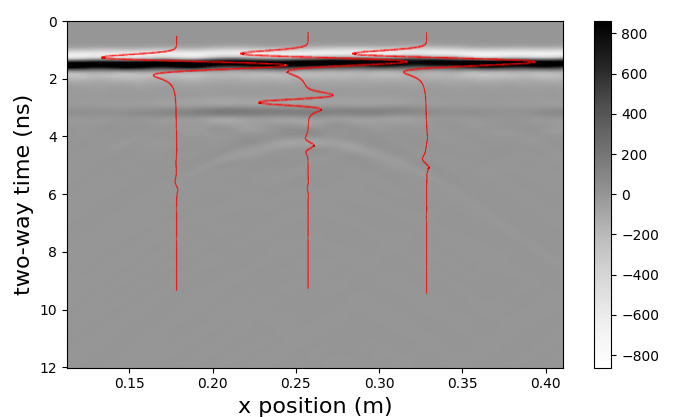
\includegraphics[width=1.0\linewidth]{figures/originalBScan.png}
  
  \caption{\\Generator and Discriminator Architecture}
  \label{fig:originalBscan}
\end{figure}

\hspace{0.5in}We re-size the B-scan to $(256,256)$ with hamming interpolation. This centers the hyperbola, and ensures the the height and width dimensions are divisible by 2 for simplicity in upsampling $N(0,1)$ in the generator and downsampling $G(z)$ in the discriminator. When producing the gprMax A-scans, we use dielectric properties that include three different pipe materials, metallic, plastic and concrete with radius ranging from 2 - 80mm, time window of 12e-9, and ricker waveform 1.5 GHz. The materials are used as classes, which allow us to condition the generator and identify the material with the object detection model.
\vspace{0.5\baselineskip}

\begin{figure}[H]
  \centering
  \begin{subfigure}[b]{0.45\linewidth}
    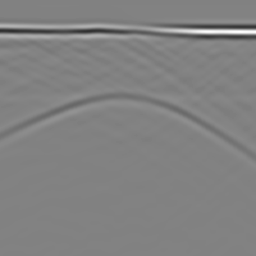
\includegraphics[width=\linewidth]{figures/peplinski_post.png}
    \caption{Time Domain}
  \end{subfigure}
  \begin{subfigure}[b]{0.45\linewidth}
    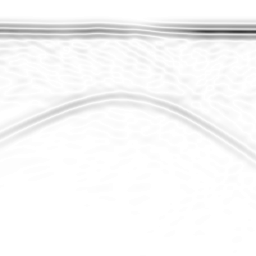
\includegraphics[width=\linewidth]{figures/frequency_post.png}
    \caption{Frequency Domain}
  \end{subfigure}
  
  \caption{\\Time and Frequency Domain Training Data Example}
  \label{fig:training_examples}
\end{figure}

\section{Challenges with Using GprMax}
\hspace{0.5in}First, it is necessary to mention that GprMax is a wonderful project and can do some really great things. However, using GprMax as a source for training data did not come without a set of challenges. The python interface is clunky and the documentation outlines only the most basic software features. The user is bound to a command line interface in python. This forces the user to sequentially generate each B-scan from the command line. Even with CUDA support, large models can take up to four hours on an Nvidia GTX 1080Ti. Now, imagine that the user wanted to generate one thousand B-scans. This would consume a great amount of the users time. An important note is that generation of many B-scans with varying features is possible. However, this task is left up to adding blocks of python in text files which has its flaws. For a solution to this we took a few steps to making this process user friendly. First, we managed to script the systematic of synthesis of B-scans with random sampling of feature combinations strictly in python without the use of the command line interface. Additionally, this can be accomplished in a Jupyter notebook though is not recommended for long generation sessions. Another solution was greatly reducing the model size. Unfortunately, this is a scaled down approach. Therefore, the models are not to the scale of real world scenarios. This relates to the aforementioned generation time. Fortunately, we were able to use the cluster at the SimCenter. In doing this, we were able to distribute the generation jobs across multiple GPU's and greatly reduce the time to generate a single B-scan to roughly three minutes. Figure \ref{fig:config_examlple} depicts a typical configuration file for GprMax.

\vspace{0.5\baselineskip}

\begin{figure}[H]
    \centering
    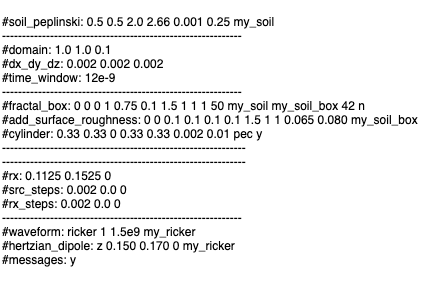
\includegraphics[width=\linewidth]{figures/config_example.png}
    
    \caption{\\GprMax Config File Example}
    \label{fig:config_examlple}
\end{figure}

\section{GAN Architecture}
\hspace{0.5in}The architecture proposed is a deep convolutional structure. Previous work suggested that a convolution with the filter with dimension of (5,5) is superior to other options for the modeling of ground penetrating radar data \cite{5x5}. Therefore, we set the kernel size of all convolutions to 5 by 5. The generator, is conditioned to upsample a noise vector into a class from a supervised label. This is accomplished by introducing a label embedding vector and concatenating it with the posterior of the generator \cite{CGAN}. From this output, we calculate Wasserstein loss with gradient penalty \cite{WGAN-GP} against the true image. The discriminator is used to determine validity of the generated output by directly comparing the two images. We calculate the Wasserstein distance between both real and fake images. In addition, the discriminator is trained to produce a predicted label for the generated image. For this output, we calculate categorical cross entropy between the predicted label and the true label. To improve overall model quality, we apply a Frequency domain loss function to $G(z)$.x 

\subsection{Generator Architecture}
 \hspace{0.5in}Table \ref{tab:gen} depicts the architecture of the generator. As depicted, the generator takes the inputs of a random noise vector and a label for the desired class. The label in then passed through an embedding layer which allows for multiplication with the noise tensor. This is the vital step for the introduction of class conditioning and leaves us with a single input for the remaining layers. Next, the combined input is passed through a dense layer which gives us the dimensonality to be able to reshape the tensor into the 3-Dimensional shape of an image. From this point, we begin the upsampling process. We derive the upsampling method from \cite{lapgan}, which indicates that many upsampling layers are favorable. In addition, we pass the upsampled vector though a convolution layer. This allows us to retain only the important information that we upsampled. Each time the input passes though an upsampling layer it doubles in size. The output is then activated with ReLU \cite{relu} and then passed through a batch normalization layer for regularization. We continue this process until the generator input is the same size as our target image. Finally, a Tanh \cite{tanh} activation is applied to restrict the output to the range (-1, 1). The important part of the generator is that we want to learn the transformation of a noise vector into an image. We use a gaussian noise vector because it contains the least amount of prior knowledge \cite{Goodfellow-et-al-2016}. Therefore, the primary learning objective is not what the generator learns from the noise vector, but how we can exploit the functional approximation property of neural networks to transform the noise vector into an image.  


\begin{center}
    \begin{table}[H]
        \centering
        \caption{\\Generator Architecture}
        \begin{tabular}{c|c}
            Operation & Output Shape \\
            \hline
            Input $N(0,1)$ & (n, 100) \\
            Label        & (n, 1) \\
            Embedding    & (n, 1, 100)\\
            Flatten      & (n, 100) \\
            Multiply     & (n, 100) \\
            Dense(8*8*128)       & (n, 8192) \\
            Reshape(8, 8, 128)      & (n, 8, 8, 128) \\
            BatchNormalization(momentum=0.8) & (n, 8, 8, 128)\\
            ConvTranspose2D(filters=128, kernel-size=5) & (n, 16, 16, 128) \\
            Conv2D(filters=256, kernel-size=5, strides=1)       & (n, 16, 16, 256) \\
            ReLU         & (n, 16, 16, 256)\\
            BatchNormalization(momentum=0.8) & (n, 16, 16, 256)\\
            ConvTranspose2D(filters=256, kernel-size=5) & (n, 32, 32, 256)\\
            Conv2D(filters=128, kernel-size=5, strides=1)      & (n, 32, 32, 128)\\
            ReLU         & (n, 32, 32, 128)\\
            BatchNormalization(momentum=0.8) & (n, 32, 32, 128)\\
            ConvTranspose2D(filters=128, kernel-size=5) & (n, 64, 64, 128)\\
            Conv2D(filters=64, kernel-size=5, strides=1) & (n, 64, 64, 64)\\
            ReLU         & (n, 64, 64, 64)\\
            BatchNormalization(momentum=0.8) & (n, 64, 64, 64)\\
            ConvTranspose2D(filters=64, kernel-size=5) & (n, 128, 128, 64)\\
            Conv2D(filters=32, kernel-size=5, strides=1)       & (n, 128, 128, 32)\\
            ReLU         & (n, 128, 128, 32)\\
            BatchNormalization(momentum=0.8) & (n, 128, 128, 32)\\
            ConvTranspose2D(filters=32, kernel-size=5) & (n, 256, 256, 32)\\
            Conv2D(filters=16, kernel-size=5, strides=1)       & (n, 256, 256, 16)\\
            ReLU         & (n, 256, 256, 16)\\
            BatchNormalization(momentum=0.8) & (n, 256, 256, 16)\\
            Conv2D(filters=1, kernel-size=5, strides=1)       & (n, 256, 256, 1)\\
            Tanh         & (n, 256, 256, 1)\\
        \end{tabular}
        \label{tab:gen}
    \end{table}
\end{center}


\subsection{Discriminator Architecture}
\hspace{0.5in}Table \ref{tab:disc}, is an example of the discriminator architecture. The discriminator accepts a tensor in the shape of a real image (256, 256, 1). During training, it receives both real and fake images and directly compares the two. This feedback is used to condition the generator to make better images. We use LeakyReLU\cite{leaky_relu} activation to reduce mode collapse, because the gradient after this activation is never 0. The downsampling pattern is a reversed version of the upsampling pattern in the generator. This adds additional balance to the training process which produces additional stability. Furthermore, we flatten the tensor before it enters the final Dense layer. This can be thought of as a summary of the information learned in the previous layers. Note, there is not a non-linearity applied to the output of the final layer. This is used for direct comparison with the real image. 


\begin{center}
    \begin{table}[H]
        \centering
        \caption{\\Discriminator Architecture}
        \begin{tabular}{c|c}
             Operation & Output Shape \\
             \hline
             Input & (n, 256, 256, 1)\\
             Conv2D(filters=16, kernel-size=5, strides=2) & (n, 128, 128, 16)\\
             LeakyReLU(alpha=0.3)         & (n, 128, 128, 16)\\
             Conv2D(filters=32, kernel-size=5, strides=2) & (n, 64, 64, 32)\\
             LeakyReLU(alpha=0.3)         & (n, 64, 64, 32)\\
             Conv2D(filters=64, kernel-size=5, strides=2) & (n, 32, 32, 64)\\
             LeakyReLU(alpha=0.3)         & (n, 32, 32, 64)\\
             Conv2D(filters=128, kernel-size=5, strides=2) & (n, 16, 16, 128)\\
             LeakyReLU(alpha=0.3)         & (n, 16, 16, 128)\\
             Conv2D(filters=256, kernel-size=5, strides=2) & (n, 8, 8, 256)\\
             LeakyReLU(alpha=0.3)         & (n, 8, 8, 256)\\
             Flatten           & (n, 16384)\\
             Dense(1)             & (n, 1)\\
        \end{tabular}
        \label{tab:disc}
    \end{table}
\end{center}

\subsection{Wasserstein Loss}
\hspace{0.5in}To minimize the dissimilarity between $G(z)$ and $y$ we use Wasserstein Loss \cite{WGAN}. Likewise, this loss binds the discriminator. However, we include gradient penalty introduced in \cite{WGAN-GP} to improve training stability.

\begin{equation}
\label{eq:wasserstein}
        W(p_r, p_g) = \max_{w \in W} \mathbb{E}_{x \sim p_r}[f_w(x)] - \mathbb{E}_{z \sim p_r(z)}[f_w(g_\theta(z))]
\end{equation}

\hspace{0.5in}The final loss of the discriminator is defined by Equation (\ref{eq:wass-gp}) which includes the penalty term. This penalty term, proposed in \cite{WGAN-GP}, is an improvement on the gradient clipping outlined in \cite{WGAN}.

\begin{equation}
\label{eq:wass-gp}
    L = \mathbb{E} {\tilde{x} \sim \mathbb{P}_g} [D_{w}(\tilde{x})] - [D_{w}(x)] + \lambda(\|{\nabla_{\hat{x}} D_{w}(\hat{x})}\|_{2} - 1)^2
\end{equation}



\subsection{Frequency Domain Loss}
\hspace{0.5in}In Equation (\ref{eq:time-sequence-loss}), $\phi$ represents the B-scan frequency transformation outlined in \cite{ZHANG-2017} with some minor modifications. Each A-scan that is contained in the B-scan has a \acrfull{stft} \cite{stft} with 1024 FFT bins and 16 segment size applied. From these transforms, we take the max frequency from each A-scan. The max frequencies are then concatenated back together to form a Frequency B-scan. We do take the transformation a step further, by converting the Frequency B-scan to gray-scale. This allows for a 1:1 comparison with time domain B-scans. Furthermore, we are able to use the same number of channels in the model architecture.

\begin{equation}
\label{eq:time-sequence-loss}
    % should most likely be E(x, G(z)) but I'm still verifying.
    % we already defined Wasserstein it actually may be clearer to
    % define time-freq loss as W(\phi{x}, \phi{G(z)})
    \mathbb{E}_{(x, z) \sim \mathbb{P}}\Big[ \big|\big| \phi(x) - \phi(G(z)) \big|\big| \Big]
\end{equation}

\subsection{Training Algorithm}
\hspace{0.5in}Algorithm \ref{alg} is the process we follow for training the GAN model. This process does not differ greatly from \cite{WGAN-GP}. However, we do make some modifications. The first modification is we adopt a faster $\alpha$ for Adam \cite{ADAM}. We found the original learning rate as specified in the paper to cause slower convergence. We also add \ref{eq:time-sequence-loss} to line 9. This loss is added directly to the respective Wasserstein losses. We minimize the weighted sum of all losses for the generator and discriminator individually. The algorithm begins with samples of real data and latent variable. For each iteration of the training loop, the discriminator is updated a total of five times for each generator update. This is specified by the $n_{critic}$ argument, which is consistent in naming with the original paper. 


\begin{algorithm}[H]
  \caption{WGAN with gradient penalty. \\
  We use default values of $\lambda =10$, $n_{critic} = 5$, $\alpha = 0.0003$}\label{euclid}
  
  \textbf{Require:} The gradient penalty coefficient $\lambda$, the number of critic iterations per generator $n_{critic}$, the batch size $m$, Adam hyper-parameter $\alpha$.



\textbf{Require:} initial critic parameters $w_{0}$, initial generator parameters $\theta_{0}$.
  \begin{algorithmic}[1]
   
      \While{validation loss is still decreasing}
        \For{\texttt{t=1,...,$n_{critic}$}}
            \For{\texttt{i=1,...,$m$}}
                \State Sample B-scan $x \backsim \mathbb{P} _{r}$, latent variable $z \backsim p(z)$
                \State $\Tilde{x} \xleftarrow[]{}G_{0}(z)$
                \State $\hat{x} \xleftarrow{}\epsilon x + (1 - \epsilon) \tilde{x}$
                \State $L^{(i)} \xleftarrow{} D_{w}(\tilde{x}) - D_{w}(x) + \lambda(\|{\nabla_{\hat{x}} D_{w}(\hat{x})}\|_{2} - 1)^2$
                \State \colorbox{yellow}{$L_{2}^{(i)} \xleftarrow{} \Big[ \big|\big| \phi(x) - \phi(G(z)) \big|\big| \Big]$}
            \EndFor
            \State $w \xleftarrow{} Adam (\nabla_{w} \frac{1}{m} \sum_{i=1}^{m} L^{(i)}, w, \alpha)$
        \EndFor
        \State Sample a batch of latent variable \{${z^{(i)}}$\}$_{i=1}^{m} \backsim p(z)$
        \State $\theta \xleftarrow{} Adam (\nabla_{w} \frac{1}{m} \sum_{i=1}^{m} -D_{w}(G_{\theta}(z)), \theta, w, \alpha)$
      \EndWhile\label{euclidendwhile}
    %\EndProcedure
  \end{algorithmic}
  \label{alg}
\end{algorithm}

\section{Object Identification Model}
\hspace{0.5in}We train a separate auxiliary classifier to predict the object in the image. This is a basic classifier that uses cross entropy to create a separation boundary between classes. The architecture consists of two convolution layers that lead into a fully connected layer. The output of the final fully connected layer is activated with softmax to generate a categorical probability distribution. The loss function \ref{eq:cross-entropy} is traditional categorical cross entropy.

\begin{center}
    \begin{align}
    \label{eq:cross-entropy}
        -\sum_{c=1}^My_{o,c}\log({\hat{y}})
    \end{align}
\end{center}

\hspace{0.5in}We apply this loss to both the Time B-scan and Frequency B-scan to maximize the probability of a correct class prediction. Figure \ref{tab:single_classifier} depicts the basic classifier architecture. The basic classifier has two convolution layers, both activated with Leaky ReLU \cite{leaky_relu}. We use this opposed to traditional ReLU to mimic the architecture of the discriminator. In the initial tests we sought to use the discriminator as the classifier. However, this leads to extreme over fitting in the discriminator and poor performance for the classification task. Moreover, this also had a negative effect in the adversarial game, with the generator being able to constantly fool the discriminator. An important note in using a separate classifier is that this simple architecture can be a stand in for more complex object detection models such as Faster-RCNN\cite{Faster-RCNN} or Mask-RCNN\cite{Mask-RCNN}. This was an additional reason for not using the discriminator as the object detection model. To enable the use of the Time B-scan and Frequency B-scan, the architecture has a slight modification as depicted in Figure \ref{tab:combined_classifier}. The additional fully connected layer allows us to calculate a separate loss for the Frequency B-scan which is useful in training. 


\begin{center}
    \begin{table}[H]
        \centering
        \singlespacing
        \caption{\\Single Classifier Architecture}
        \begin{tabular}{c|c}
            Operation & Output Shape \\
            \hline
            Input B-scan & (n, 256, 256, 1) \\
            Conv2D(filters=2, kernel size=1, strides=2) & (n, 128, 128, 2)\\
            LeakyReLU(alpha=0.3) & (n, 128, 128, 2) \\
            Conv2D(filters=4, kernel size=1, strides=2) & (n, 64, 64, 4)\\
            LeakyReLU(alpha=0.3) & (n, 64, 64, 4)\\
            Flatten & (n, 16384) \\
            Dense & (n, 3) \\
        \end{tabular}
        \label{tab:single_classifier}
    \end{table}
\end{center}
\begin{center}
    \begin{table}[H]
        \centering
        \caption{\\Combined Classifier Architecture}
        \begin{tabular}{c|c}
            Operation & Output Shape \\
            \hline
            Input Time B-scan & (n, 256, 256, 1)\\
            Input Frequency B-scan & (n, 256, 256, 1)\\
            SingleClassifier(Time B-scan) & (n, 64, 64, 4)\\
            SingleClassifier(Frequency B-scan) & (n, 64, 64, 4)\\
            Multiply & (n, 64, 64, 4)\\
            Flatten & (n, 16384) \\
            Dense & (n, 3) \\
        \end{tabular}
        \label{tab:combined_classifier}
    \end{table}
\end{center}

\hspace{0.5in}The auxiliary classifier is trained in three scenarios. The first, data containing only images from gprMax are adopted. We use this performance as a baseline to compare our other experiments. The second, we use the full gprMax generated dataset with additional GAN generated images. Finally, we add a concurrent frequency domain optimization function to the generator, then train the object detection model to identify cylinder material from the b-scan with the assistance of information from the frequency representation.